\subsection*{Problema y modelo}
El problema trata sobre un salón de exposiciones que cuenta con una cantidad dada de
bombillas de luz (se supone que la única fuente de luz es esta) que son fuentes de
luz puntual, y una cantidad dada de columnas, que están ubicadas de forma que no
intersecan la pared ni entre ellas, pero sí pueden tocarse. Las bombillas de luz están
ubicadas de forma que no tocan ninguna columna ni la pared. El escenario se presenta
en dos dimensiones, visto desde arriba (desde el techo del salón). Dado un salón como
el descripto, queremos saber cuál es el perímetro de la pared que cuenta con iluminación.
Se supone que la sombra no sufre difusión ni hay fenómenos reflexión de luces.

Representamos la bombilla como un punto $(x,y)$ en el plano, las columnas como circulos
$(x,y,r)$ de centro $(x,y)$ y radio $r$, y las paredes como 4 segmentos: $\overline{AB}$,
$\overline{BC}$, $\overline{CD}$, $\overline{DA}$, siendo

\vspace{0.2cm}
$A = (0, 0)$

$B = (X, 0)$

$C = (X, Y)$

$D = (0, Y)$
\vspace{0.2cm}

con X e Y dados por el enunciado, por ejemplo:

\begin{figure}[H]
\centering
\label{bl_1}
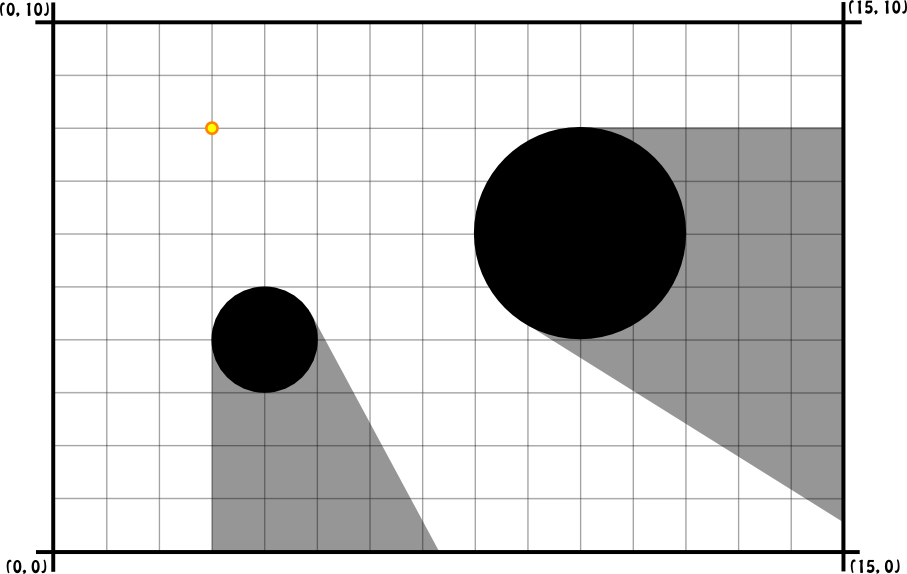
\includegraphics[scale=1.0]{./figuras/bl_1.png}
\caption{Ejemplo del modelo}
\end{figure} 

\subsection*{Solución}

Como dice el enunciado, un punto $p$ dado del perímetro de la pared es iluminado si
existe un segmento de línea (un rayo de luz) que comienza en una bombilla de luz, finaliza
en p y no toca o pasa a través de alguna columna, por lo tanto:
\begin{itemize}
\item Una cierta porción de la pared está iluminada si alguna bombilla la ilumina (por lo tanto
no está iluminada si ninguna bombilla la ilumina, es decir, si todas las columnas proyectan una
sombra sobre esta parte de la pared).
\item La sombra que proyecta una columna $c$ a partir de la luz que incide una bombilla $b$
depende de las tangentes del círculo (que representa la columna $c$) que pasan por el punto
$b$, de forma que, detrás de la columna (visto desde la bombilla) desde una
tangente a la otra se proyectará sombra (si ninguna otra bombilla ilumina la porción) y todo
lo demás se iluminará (si la luz no cruza ninguna otra columna).
\end{itemize}

La solución que presentamos aprobecha estas características. La idea básica del algoritmo es
tomar cada luz y para cada una de ellas calcular las porciones de pared que ilumina.
Para esto recorremos todas las columnas y calculamos la sombra que genera la luz con cada columna
usando las tangentes de la columna que pasan por el punto que representa la luz,
y con estas sombras generamos un conjunto de sombras para cada luz.

Para describir el conjunto de sombras vemos la pared como un único intervalo $(0, 2X + 2Y)$, como
si estuviésemos recorriendo las paredes en sentido antihorario, comenzando desde la pared inferior,
por ejemplo:

\begin{figure}[H]
\centering
\label{bl_2}
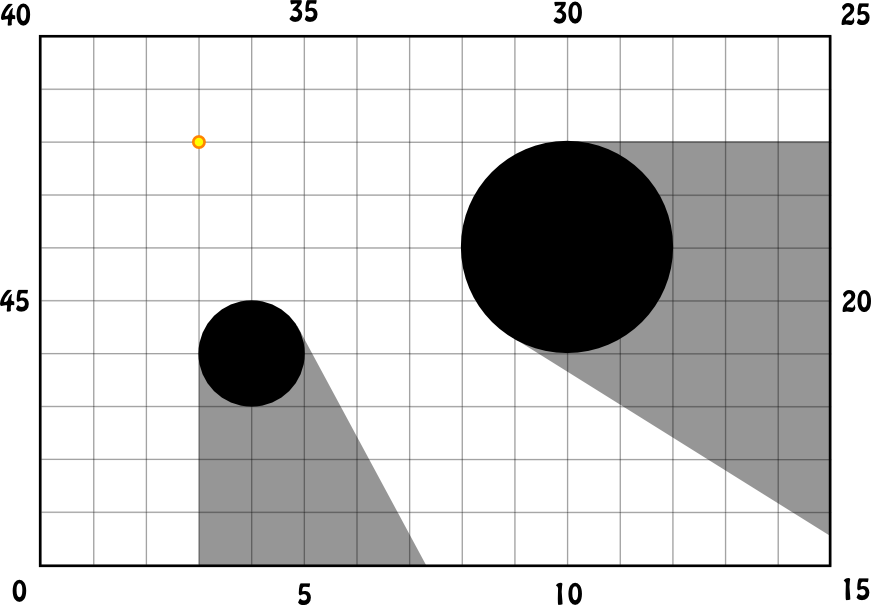
\includegraphics[scale=1.0]{./figuras/bl_2.png}
\caption{Pared vista como un intervalo en R}
\end{figure}

y las sombras como subintervalos del mismo (para ver cómo se hace esta traducción de los segmentos
de pared a un intervalo ir a la sección de Cálculo de sombras).
El complemento de un conjunto de sombras son los intervalos de pared iluminada, y resulta simple
de calcular si antes nos aseguramos que para este conjunto de intervalos todos sus elementos tengan
intersección vacía. Para esto ``comprimimos'' el conjunto (realizamos la union entre intervalos de
intersección no vacía) y luego su complemento.

A continuación unimos todos los conjuntos de intervalos iluminados por las bombillas, formando
otro conjunto. Nuevamente, es simple calcular la longitud de las porciones iluminadas del salón
si nos aseguramos que para este conjunto todos sus elementos tengan intersección vacía. Para esto
``comprimimos'' el conjunto en el mismo sentido que antes y calculamos el resultado del problema,
que es:

\vspace{0.2cm}
\begin{center}$\displaystyle\sum_{e \in intIlum}e_y - e_x$\end{center}
\vspace{0.2cm}

Notar que $(\forall e \in intIlum)e_y > e_x$, por construcción (ver la sección de
Cálculo de sombras).

Para contemplar el error de las operaciones entre flotantes utilizamos un $\epsilon = 0.0000001$, 
de modo que dos flotantes $x_1$ y $x_2$ son considerados iguales si: $abs(x_1 - x_2) < \epsilon$.

\subsection*{Cálculo de sombras}
Dada una luz $L = (l_x, l_y)$ y una columna $C = (c_x, c_y, c_r)$ para calcular la porción sobre
la que se proyecta una sombra consideramos los triángulos que se forman como muestra el siguiente
gráfico:

\begin{figure}[H]
\centering
\label{bl_3}
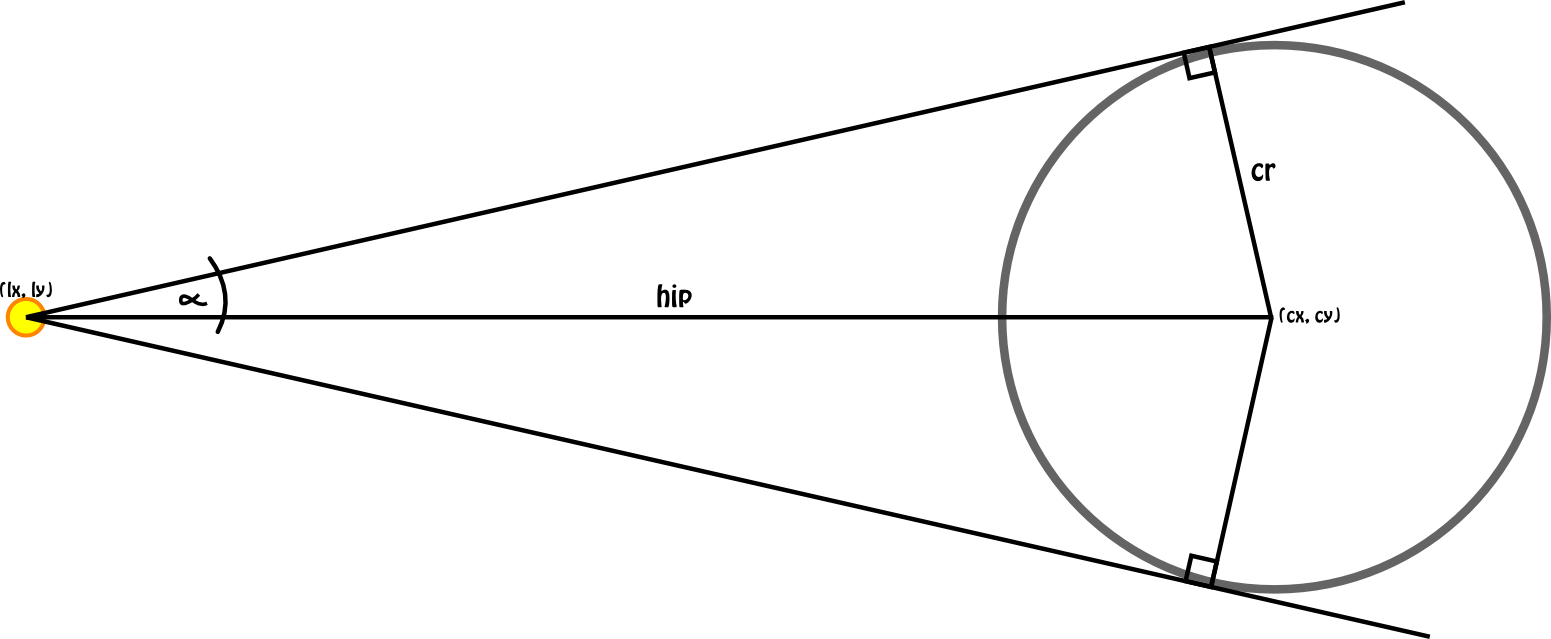
\includegraphics[scale=1.0]{./figuras/bl_3.png}
\caption{los rayos de luz que inciden en la columna}
\end{figure} 

y con esto:

\begin{itemize}
\item calculamos el vector $v = (c_x - l_x, c_y - l_y)$ que es el que va desde la luz hacia
el centro de la columna.
\item el largo de la hipotenusa coincide con la norma del vector $v$, por lo tanto calculamos $|v|$.
\item dado que son triángulos rectángulos, calculamos el seno de alfa como
$\displaystyle\frac{c_r}{|v|}$ por trigonometría.
\item por la propiedad $\sin^2(\alpha) + \cos^2(\alpha) = 1$, despejamos y calculamos $\cos(\alpha)$
\item \textbf{calculamos las tangentes:} rotamos el vector $v$ un ángulo $\alpha$ y un ángulo
$-\alpha$, teniendo en cuenta las propiedades $\sin(-\alpha) = -\sin(\alpha)$ y
$\cos(-\alpha) = \cos(\alpha)$, multiplicando:

\vspace{0.2cm}
\begin{center}
$\left(
\begin{array}{cc}
\cos(\alpha) & -\sin(\alpha) \\
\sin(\alpha) & \cos(\alpha) \\
\end{array}
\right)
v = t_1$
\hspace{1cm}
$\left(
\begin{array}{cc}
\cos(\alpha) & \sin(\alpha) \\
-\sin(\alpha) & \cos(\alpha) \\
\end{array}
\right)  
v = t_2$
\end{center}
\vspace{0.2cm}

esto resulta en dos vectores $t_1$ y $t_2$. A partir de estos vectores consideramos las semirrectas
$st_1$ y $st_2$, ambas de origen $(l_x, l_y)$ y con vectores generadores $t_1$ y $t_2$
respectivamente. Las semirrectas las representamos en su forma vectorial.
\item \textbf{calculamos los puntos de intersección $(x_1, y_1)$ y $(x_2, y_2)$ de las semirrectas
$st_1$ y $st_2$ respectivamente con los segmentos que representan la pared:} ver sección
``Intersección entre semirrecta y segmento''.
\item \textbf{a partir de los puntos de intersección calculamos el intervalo de sombra}
considerando los 4 segmentos de la pared como un único segmento del largo del perímetro,
de la siguiente forma:

sea la función de $R^2 \times R$

\vspace{0.2cm}
\begin{center}
\[ f(x, y) = \left\{
               \begin{array}{llll}
				 $x$ & \mbox{si $0 \le x < X \wedge y = 0$} \\
				 $X + y$ & \mbox{si $x = X \wedge 0 \le y < Y$} \\
				 $2X + Y - x$ & \mbox{si $0 < x \le X \wedge y = Y$} \\
				 $2X + 2Y - y$ & \mbox{si $x = 0 \wedge 0 < y \le Y$}
			   \end{array}
			 \right.
\]
\end{center}
\vspace{0.2cm}

\end{itemize}

entonces el intervalo de sombra lo definimos como $(f(x_1,y_1), f(x_2,y_2))$ si
$f(x_1,y_1) \le f(x_2,y_2)$, sino definimos la sombra con dos intervalos: $(0, f(x_2,y_2))$ y
$(f(x_1,y_1), 2X + 2Y)$. Este último caso sucede cuando está el punto $(0,0)$ entre las 
semirrectas tangentes a la columna.

\subsection*{Intersección entre semirrecta y segmento}

Dada una semirrecta de origen $(x_1, y_1)$ y vector generador $(x_2 - x_1, y_2 - y_1)$ y un
segmento $<(w_1, z_1), (w_2, z_2)>$:
\begin{itemize}
\item construímos, con el segmento, una semirrecta de origen $(w_1, z_1)$ y vector generador
$(w_2 - w_1, z_2 - z_1)$.
\item calculamos la intersección entre estas semirrectas, y para esto hacemos el mismo cálculo que
para las rectas, y luego restringimos el resultado, de modo que las rectas serían

\vspace{0.2cm}
$recta_1 = (x_1, y_1) + t(x_2 - x_1, y_2 - y_1)$

\vspace{0.1cm}
$recta_2 = (w_1, z_1) + s(w_2 - w_1, z_2 - z_1)$
\vspace{0.2cm}

\item calculamos la intersección entre las semirrectas resolviendo el sistema 

\vspace{0.2cm}
\begin{center}$(x_1 + t(x_2 - x_1), y_1 + t(y_2 - y_1)) = (w_1 + s(w_2 - w_1), z_1 + s(z_2 - z_1))$\end{center}
\vspace{0.2cm}

Despejando nos queda

\vspace{0.2cm}
\begin{center}
$s = \displaystyle\frac{(w_1 - x_1)(y_2 - y_1) + (y_1 - z_1)(x_2 - x_1)}
                       {(x_2 - x_1)(z_2 - z_1) - (w_2 - w_1)(y_2 - y_1)}$
\end{center}
\vspace{0.2cm}

Por lo tanto este sistema no tiene solución o tiene infinitas soluciones si las semirrectas son
paralelas (infinitas soluciones si las rectas están una encima de la otra y no tiene solución si
son paralelas pero no están encimadas), lo que quiere decir que el determinante de la matriz
formada por los dos vectores generadores

\vspace{0.2cm}
\begin{center}
$\vline
\begin{array}{cc}
x_2 - x_1 & w_2 - w_1 \\
y_2 - y_1 & z_2 - z_1 \\
\end{array}\vline
= (x_2 - x_1)(z_2 - z_1) - (w_2 - w_1)(y_2 - y_1) = 0$
\end{center}
\vspace{0.2cm}

o sea que los vectores generadores son LD.
\end{itemize}
Sin embargo calculando la intersección entre semirrectas hay un caso borde en el que el
determinante es $0$ pero el sistema tiene una única solución: si las semirrectas tienen el mismo
origen pero sentido contrario, la intersección es el punto de origen. Para saber si tienen sentido
contrario verificamos si el producto interno entre los vectores generadores es negativo.

Si el determinante de la matriz es distinto de cero, la solución es única. Para saber cual es el
punto $p$ de intersección simplemente reemplazamos $s$ en alguna de las dos rectas con el valor
calculado.

Para saber si el punto cae sobre ambas semirrectas verificamos para cada una que el producto
interno entre el vector generador de la semirrecta y el vector que va desde el origen de la
semirrecta hacia $p$ es positivo, que es lo mismo que ver que estos vectores tienen igual sentido
que la semirrecta.

Finalmente, dado el punto de intersección, para saber si cae sobre el segmento resta verificar si
es positivo el producto interno entre el vector que va desde el punto $(w_2, z_2)$ a $(w_1, z_1)$
y el vector que va desde $(w_2, z_2)$ a $p$. Recordemos que no hace falta verificar lo mismo con el
vector que va desde $(w_1, z_1)$ a $(w_2, z_2)$, pues ya lo hicimos cuando calculamos la
intersección entre las semirrectas (el origen de una de las semirrectas era $(w_1, z_1)$).
Intuitivamente esto es lo mismo que verificar que los vectores que van desde los extremos del
segmento hacia $p$ apuntan hacia ``adentro'' del segmento.

\subsection*{Detalles de Implementación}

Fue implementada la clase \textbf{Par}, que representa un par en $R^2$. Además, para esta
estructura implementamos el operador de resta y de comparación por menor. La comparación por menor
para dos pares es

\vspace{0.2cm}
$(x_1, y_1) < (x_2, y_2) \Leftrightarrow x_1 < x_2 \vee ( abs(x_1 - x_2) < \epsilon \wedge y_1 < y_2 )$
\vspace{0.2cm}

Se implementó el método \textbf{prodInterno} que para dos pares dados devuelve el producto interno.

Se implementó la clase \textbf{Segmento} que es un par de pares.

Se implementó la clase \textbf{Semirrecta} que tiene un par que es el origen y un par que es el 
vector generador.

Se implementó la clase \textbf{Columna} que tiene tres enteros: $x$, $y$ que son el centro, y $r$
que es el radio de la columna.

Se implementó la clase \textbf{Luz} que tiene dos enteros: $x$, $y$ que es la ubicación de la luz
en los ejes XY.

Se implementó el método \textbf{interSemirrectas} que dadas dos semirrectas y un par, devuelve un
booleano que indica si existe o no intersección entre las semirrectas. Si existe intersección la
devuelve en el par, sino deja el par con los valores originales.

Se implementó el método \textbf{interSemirrectaSeg} que dada una recta, un segmento y un par,
devuelve un booleano que indica si existe o no intersección entre la semirrecta y el segmento.
Si existe intersección la devuelve en el par, sino deja el par con los valores originales.

Estos dos últimos métodos son la implementación de lo explicado en la sección ``Intersección entre
semirrecta y segmento''.

Se implementó el método \textbf{intervaloSombra} que dado un objeto Luz y un objeto Columna devuelve
un par que es el intervalo de la sombra proyectada en la pared a causa de la luz emitida por la
bombilla que incide en la columna. Este método es la implementación de lo explicado en la sección
``Cálculo de sombras'', con la diferencia que si la primer coordenada del par es mayor a la segunda
coordenada del par este método no es el responsable de partirlo, sino que lo devuelve así y luego
se parte.

Se implementó el método \textbf{comprimir} que dado un vector de pares lo modifica de modo que
al salir de la función este vector cumple que todo par de elementos tiene intersección vacía.

Se implementó el método \textbf{complemento} que dado un vector de pares, un valor mín y otro valor
máx, modifica el vector tal que si lo unimos con el vector original y luego comprimimos el
resultado sería un par $(min, max)$. Además asegura que el vector resultado cumple que todo par de
elementos tiene intersección vacía.

Se implementó el método \textbf{perimIluminado} resuelve el problema utilizando todos los métodos
anteriores (como se explicó en la sección ``Solución'').

Representamos la pared con un vector de segmentos de 4 posiciones, las columnas con un vector de 
columnas y las luces con un vector de luces.

\subsection*{Análisis de complejidad}

A continuación analizamos la complejidad del algoritmo.

Los métodos prodInterno, interSemirrectas, interSemirrectaSeg y intervaloSombra tienen complejidad 
constante, dado que sólo se realizan cálculos matemáticos y se ejecutan linealmente.

El método comprimir se puede hacer en $O(n*log(n))$, siendo n el tamaño del vector de entrada. Esto 
es porque al comprimir antes de comenzar a calcular el resultado ordenamos el vector de entrada 
($O(n*log(n))$), luego recorre linealmente el vector de pares ($O(n)$), construyendo el resultado, 
y finalmente modificamos el vector de entrada copiándole el resultado ($O(n)$).

El método complemento también se puede hacer en $O(n*log(n))$, pues utiliza comprimir y luego recorre 
linealmente el vector de pares ($O(n)$), construyendo el resultado, y finalmente modificamos el vector 
de entrada copiándole el resultado ($O(n)$).

El método perimIluminado es la raíz de todos estos métodos. Este método recorre todas las luces y 
por cada luz recorre todas las columnas.

Veamos que pasa con el ciclo que recorre todas las columnas: para cada columna se llama a 
intervaloSombra, se hace una comparación booleana y se pushean a lo sumo dos elementos detrás de un 
vector de pares, por lo que el cuerpo del ciclo que recorre todas las columnas es $O(1)$.

Veamos que pasa con el ciclo que recorre todas las luces: para cada luz se recorre todas las columnas 
y se genera un vector de pares de tamaño $C$, siendo $C$ la cantidad de columnas (el mismo C del 
enunciado). Esto cuesta $O(C*log(C))$ y pushea todos los pares resultantes de este complemento en otro 
vector de pares, lo que tiene complejidad $O(C)$.

Por lo tanto el ciclo entero que recorre las luces y columnas tiene complejidad $O(L*C*log(C))$. El 
resultado de todo este ciclo es un vector de pares que representan las porciones iluminadas de la pared, 
de tamaño máximo L*C.

A continuación se comprime el vector de pares de porciones iluminadas, lo que tiene complejidad 
$O(L*C*log(L*C))$ y resulta en un vector de tamaño máximo $C+1$. La idea intuitiva de esta cota es que 
el peor caso para el tamaño de este vector es una luz y $C$ columnas, lo que como máximo genera $C+1$ 
porciones iluminadas. Al agregar luces no agregamos sombras sino que al contrario, probablemente unimos 
partes iluminadas, lo que decrementa la cantidad de partes iluminadas.

Finalmente, se recorre este vector de porciones iluminadas ya comprimido para aumentar un acumulador que 
resulta ser la respuesta al problema, lo que tiene orden $O(C)$.

Por lo tanto, el orden del algoritmo entero es $O(L*C*log(C) + L*C*log(L*C) + C)$ que es $O(L*C*log(L*C))$.